%%%%%%%%%%%%%%%%%%%%%%%%%%%%%%%%%%%%%%%%%%%%%%%%%%%%%%%%%%%%%%%%%%%%%
%% This is a (brief) model paper using the achemso class
%% The document class accepts keyval options, which should include
%% the target journal and optionally the manuscript type. 
%%%%%%%%%%%%%%%%%%%%%%%%%%%%%%%%%%%%%%%%%%%%%%%%%%%%%%%%%%%%%%%%%%%%%
\documentclass[journal=jacsat,manuscript=article]{achemso}

%%%%%%%%%%%%%%%%%%%%%%%%%%%%%%%%%%%%%%%%%%%%%%%%%%%%%%%%%%%%%%%%%%%%%
%% Place any additional packages needed here.  Only include packages
%% which are essential, to avoid problems later. Do NOT use any
%% packages which require e-TeX (for example etoolbox): the e-TeX
%% extensions are not currently available on the ACS conversion
%% servers.
%%%%%%%%%%%%%%%%%%%%%%%%%%%%%%%%%%%%%%%%%%%%%%%%%%%%%%%%%%%%%%%%%%%%%
\usepackage[version=3]{mhchem} % Formula subscripts using \ce{}
\usepackage{algorithm}
\usepackage{algpseudocode}
\usepackage{svg}
\usepackage{amsmath}
%%%%%%%%%%%%%%%%%%%%%%%%%%%%%%%%%%%%%%%%%%%%%%%%%%%%%%%%%%%%%%%%%%%%%
%% If issues arise when submitting your manuscript, you may want to
%% un-comment the next line.  This provides information on the
%% version of every file you have used.
%%%%%%%%%%%%%%%%%%%%%%%%%%%%%%%%%%%%%%%%%%%%%%%%%%%%%%%%%%%%%%%%%%%%%
%%\listfiles

%%%%%%%%%%%%%%%%%%%%%%%%%%%%%%%%%%%%%%%%%%%%%%%%%%%%%%%%%%%%%%%%%%%%%
%% Place any additional macros here.  Please use \newcommand* where
%% possible, and avoid layout-changing macros (which are not used
%% when typesetting).
%%%%%%%%%%%%%%%%%%%%%%%%%%%%%%%%%%%%%%%%%%%%%%%%%%%%%%%%%%%%%%%%%%%%%
\newcommand*\mycommand[1]{\texttt{\emph{#1}}}

%%%%%%%%%%%%%%%%%%%%%%%%%%%%%%%%%%%%%%%%%%%%%%%%%%%%%%%%%%%%%%%%%%%%%
%% Meta-data block
%% ---------------
%% Each author should be given as a separate \author command.
%%
%% Corresponding authors should have an e-mail given after the author
%% name as an \email command. Phone and fax numbers can be given
%% using \phone and \fax, respectively; this information is optional.
%%
%% The affiliation of authors is given after the authors; each
%% \affiliation command applies to all preceding authors not already
%% assigned an affiliation.
%%
%% The affiliation takes an option argument for the short name.  This
%% will typically be something like "University of Somewhere".
%%
%% The \altaffiliation macro should be used for new address, etc.
%% On the other hand, \alsoaffiliation is used on a per author basis
%% when authors are associated with multiple institutions.
%%%%%%%%%%%%%%%%%%%%%%%%%%%%%%%%%%%%%%%%%%%%%%%%%%%%%%%%%%%%%%%%%%%%%
\author{Nicholas Runcie}
\altaffiliation{EaSTCHEM School of Chemistry, University of Edinburgh, EH9 3FJ}
\author{Antonia S.J.S. Mey}
\altaffiliation{EaSTCHEM School of Chemistry, University of Edinburgh, EH9 3FJ}
\email{antonia.mey@ed.ac.uk}
\phone{xxx}


%%%%%%%%%%%%%%%%%%%%%%%%%%%%%%%%%%%%%%%%%%%%%%%%%%%%%%%%%%%%%%%%%%%%%
%% The document title should be given as usual. Some journals require
%% a running title from the author: this should be supplied as an
%% optional argument to \title.
%%%%%%%%%%%%%%%%%%%%%%%%%%%%%%%%%%%%%%%%%%%%%%%%%%%%%%%%%%%%%%%%%%%%%
\title[SILVR: Molecular Generation for binding modes]
  {SILVR: Conditional diffusion model for molecule generation without additional training}

%%%%%%%%%%%%%%%%%%%%%%%%%%%%%%%%%%%%%%%%%%%%%%%%%%%%%%%%%%%%%%%%%%%%%
%% Some journals require a list of abbreviations or keywords to be
%% supplied. These should be set up here, and will be printed after
%% the title and author information, if needed.
%%%%%%%%%%%%%%%%%%%%%%%%%%%%%%%%%%%%%%%%%%%%%%%%%%%%%%%%%%%%%%%%%%%%%
\abbreviations{}
\keywords{ML, generative models, docking}

%%%%%%%%%%%%%%%%%%%%%%%%%%%%%%%%%%%%%%%%%%%%%%%%%%%%%%%%%%%%%%%%%%%%%
%% The manuscript does not need to include \maketitle, which is
%% executed automatically.
%%%%%%%%%%%%%%%%%%%%%%%%%%%%%%%%%%%%%%%%%%%%%%%%%%%%%%%%%%%%%%%%%%%%%
\begin{document}

%%%%%%%%%%%%%%%%%%%%%%%%%%%%%%%%%%%%%%%%%%%%%%%%%%%%%%%%%%%%%%%%%%%%%
%% The "tocentry" environment can be used to create an entry for the
%% graphical table of contents. It is given here as some journals
%% require that it is printed as part of the abstract page. It will
%% be automatically moved as appropriate.
%%%%%%%%%%%%%%%%%%%%%%%%%%%%%%%%%%%%%%%%%%%%%%%%%%%%%%%%%%%%%%%%%%%%%
\begin{tocentry}

Some journals require a graphical entry for the Table of Contents.
This should be laid out ``print ready'' so that the sizing of the
text is correct.

Inside the \texttt{tocentry} environment, the font used is Helvetica
8\,pt, as required by \emph{Journal of the American Chemical
Society}.

The surrounding frame is 9\,cm by 3.5\,cm, which is the maximum
permitted for  \emph{Journal of the American Chemical Society}
graphical table of content entries. The box will not resize if the
content is too big: instead it will overflow the edge of the box.

This box and the associated title will always be printed on a
separate page at the end of the document.

\end{tocentry}

%%%%%%%%%%%%%%%%%%%%%%%%%%%%%%%%%%%%%%%%%%%%%%%%%%%%%%%%%%%%%%%%%%%%%
%% The abstract environment will automatically gobble the contents
%% if an abstract is not used by the target journal.
%%%%%%%%%%%%%%%%%%%%%%%%%%%%%%%%%%%%%%%%%%%%%%%%%%%%%%%%%%%%%%%%%%%%%
\begin{abstract}
I'll be an abstract when I grow up. 
\end{abstract}

%%%%%%%%%%%%%%%%%%%%%%%%%%%%%%%%%%%%%%%%%%%%%%%%%%%%%%%%%%%%%%%%%%%%%
%% Start the main part of the manuscript here.
%%%%%%%%%%%%%%%%%%%%%%%%%%%%%%%%%%%%%%%%%%%%%%%%%%%%%%%%%%%%%%%%%%%%%
\section{Introduction}
- Equivariant diffusion models have been very promising in predicting 3D structures of drug-like molecules. 
- This does not make them suitable candidates for a target binding site. 
- We combine equivariant diffusion models~\cite{huang2022mdm} with Iterative latent variable refinement proposed in Denoising Diffusion probabilistic models~\cite{choi2021ilvr}.
- This allows the generation of new molecules in the shape of the binding site using information from existing fragments.
\begin{figure}
    \centering
    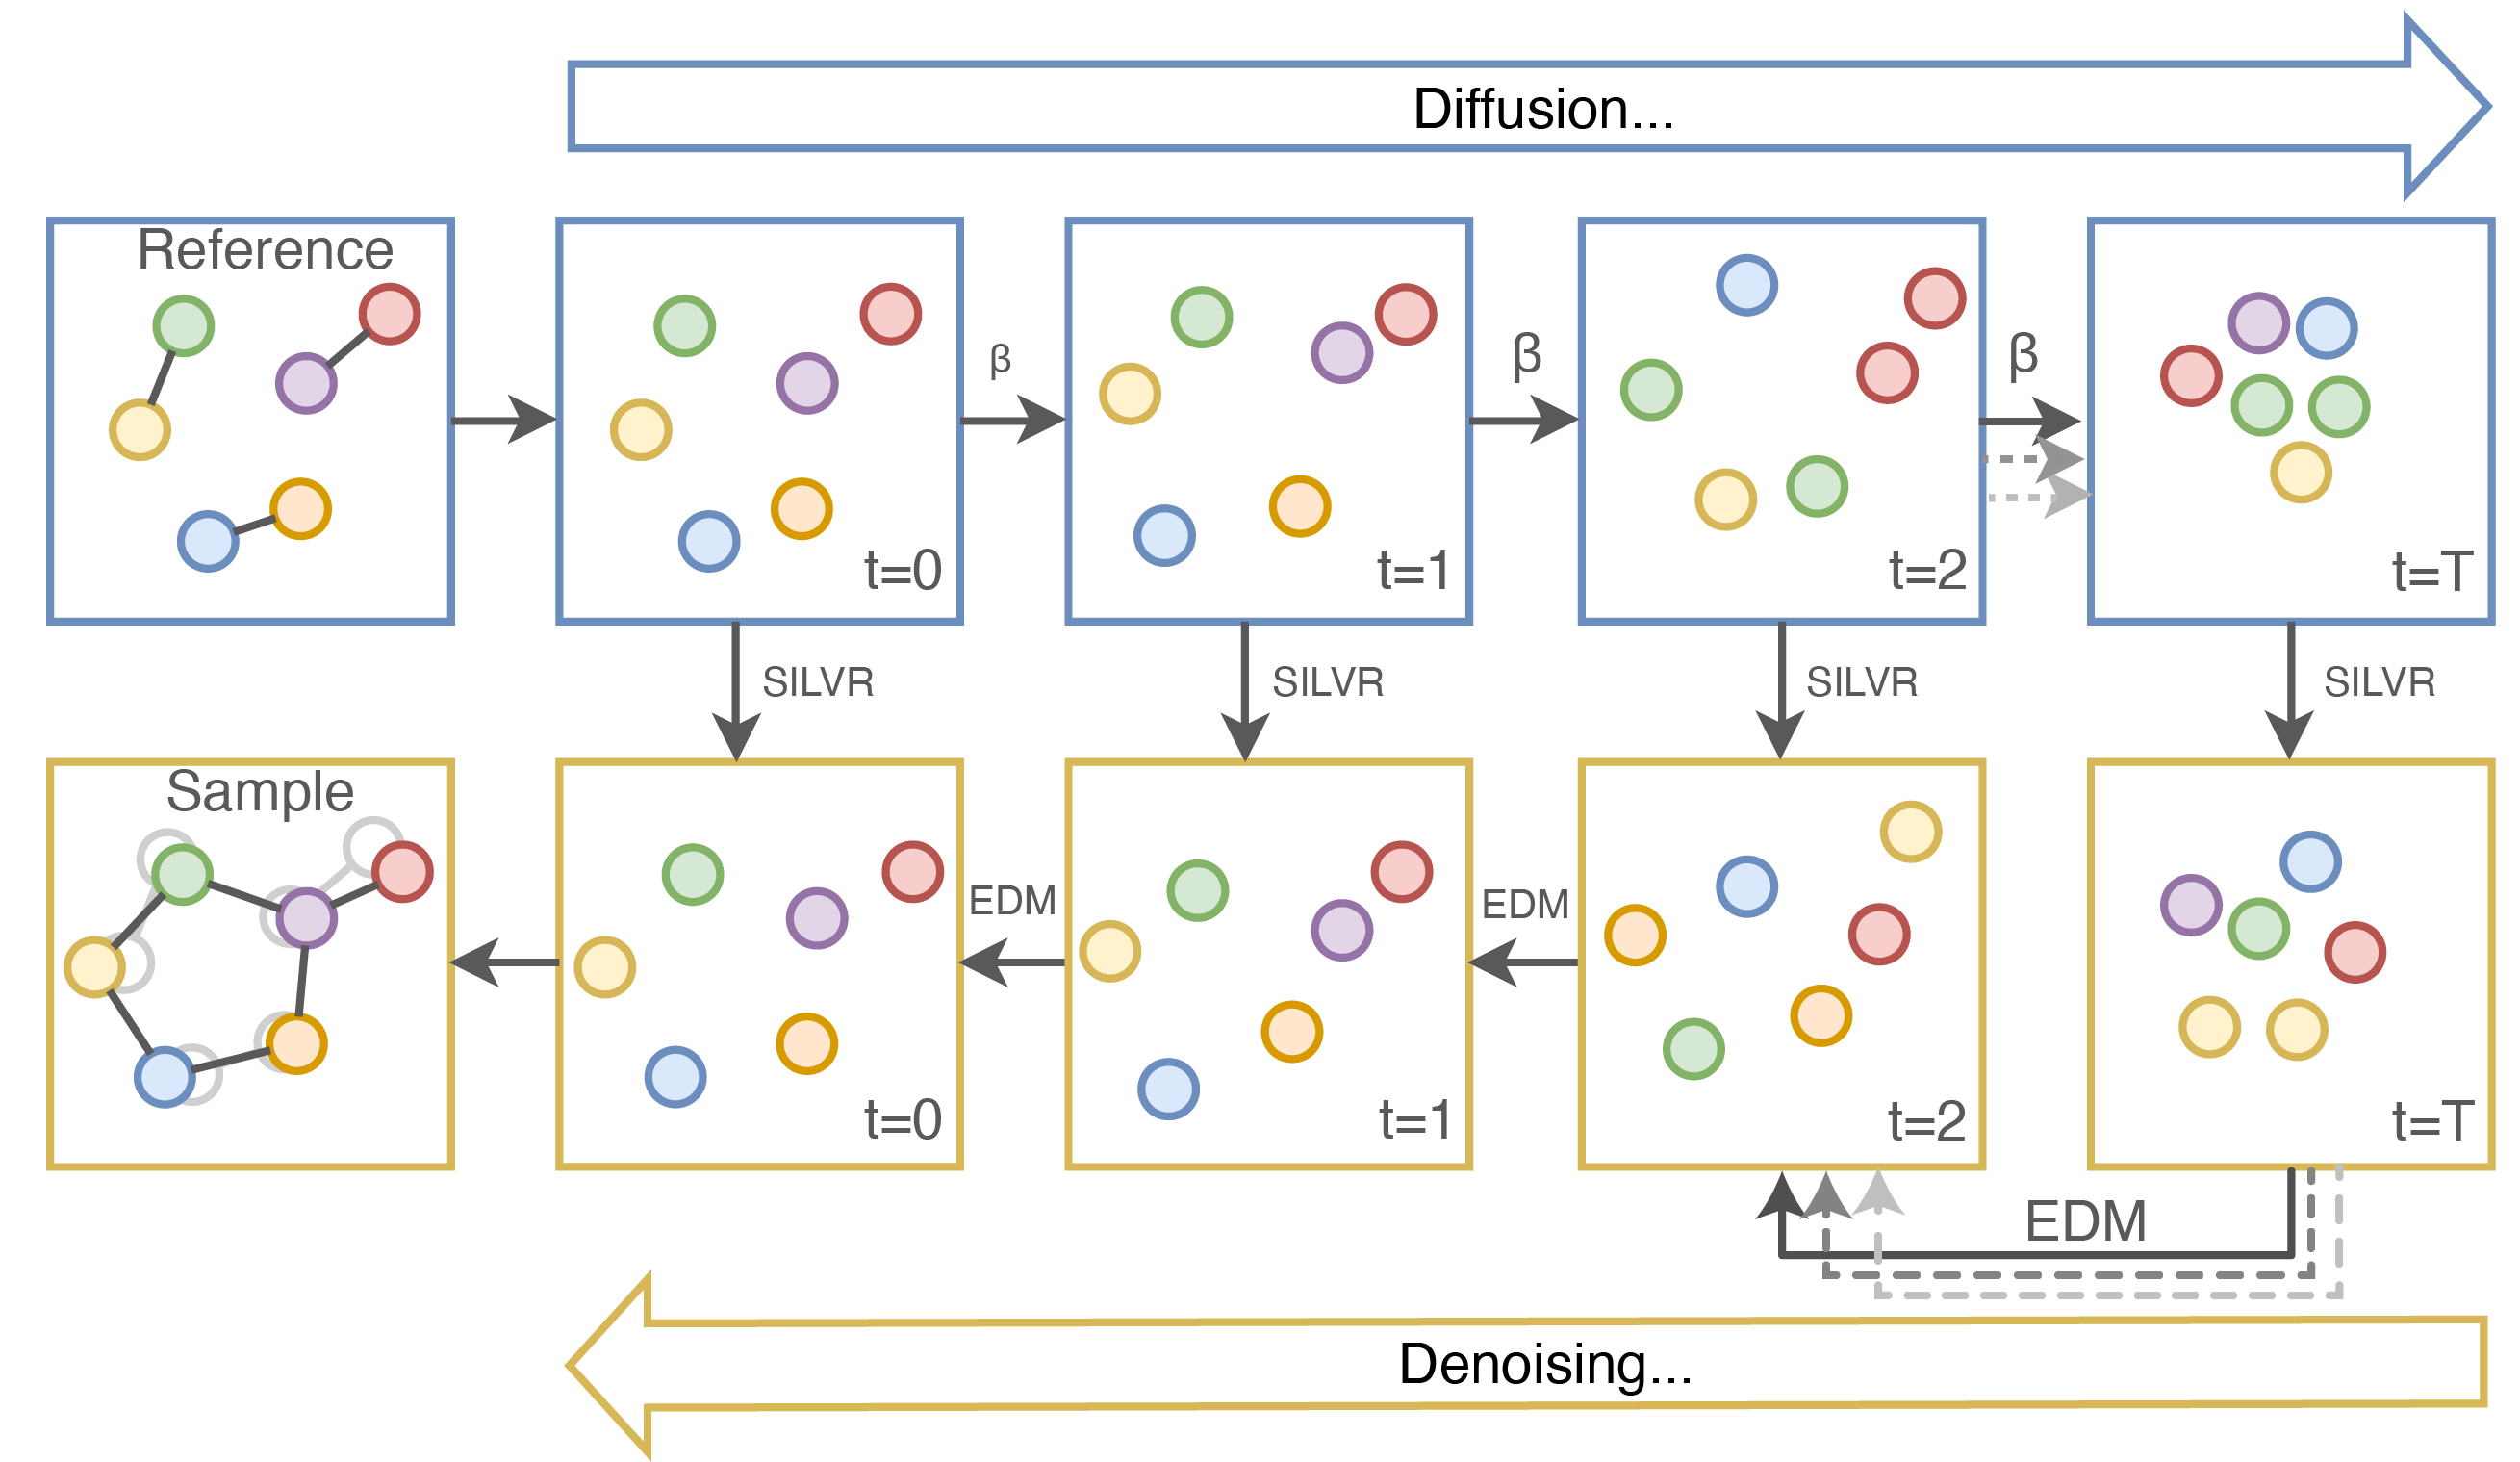
\includegraphics[width=\textwidth]{paper/Figures/Fig1/Schematic.png}
    \caption{Schematic of the equivariant diffusion model with  SILVR indicated for every denoising step.}
    \label{fig:schematic}
\end{figure}
\section{Theory}
\subsection{Unconditional Equivariant Denoising Diffusion probabilistic models}
\subsubsection*{Denoising Diffusion probabilistic models (DDPM) as generative models}
DDPMs are often used as generative models that were developed for the generation of new images~\cite{}. More recently the same idea has also been applied to molecular generation~\cite{}. The main idea behind diffusion models is for a neural network to learn the reverse of a diffusion process, often referred to as denoising to \textit{sample} a new image or new molecule. In practice this is done by training a neural network $\phi$ and generating samples $\hat{\mathbf{x}}=\psi(X_t,t)$, with $X_t$ with data $X$, noised up to time $t$.  DDPMs consist of two main parts the diffusion process and the denoising process, see the schematic in figure~\ref{fig:diffusion_schematic}.
\begin{figure}
    \centering
    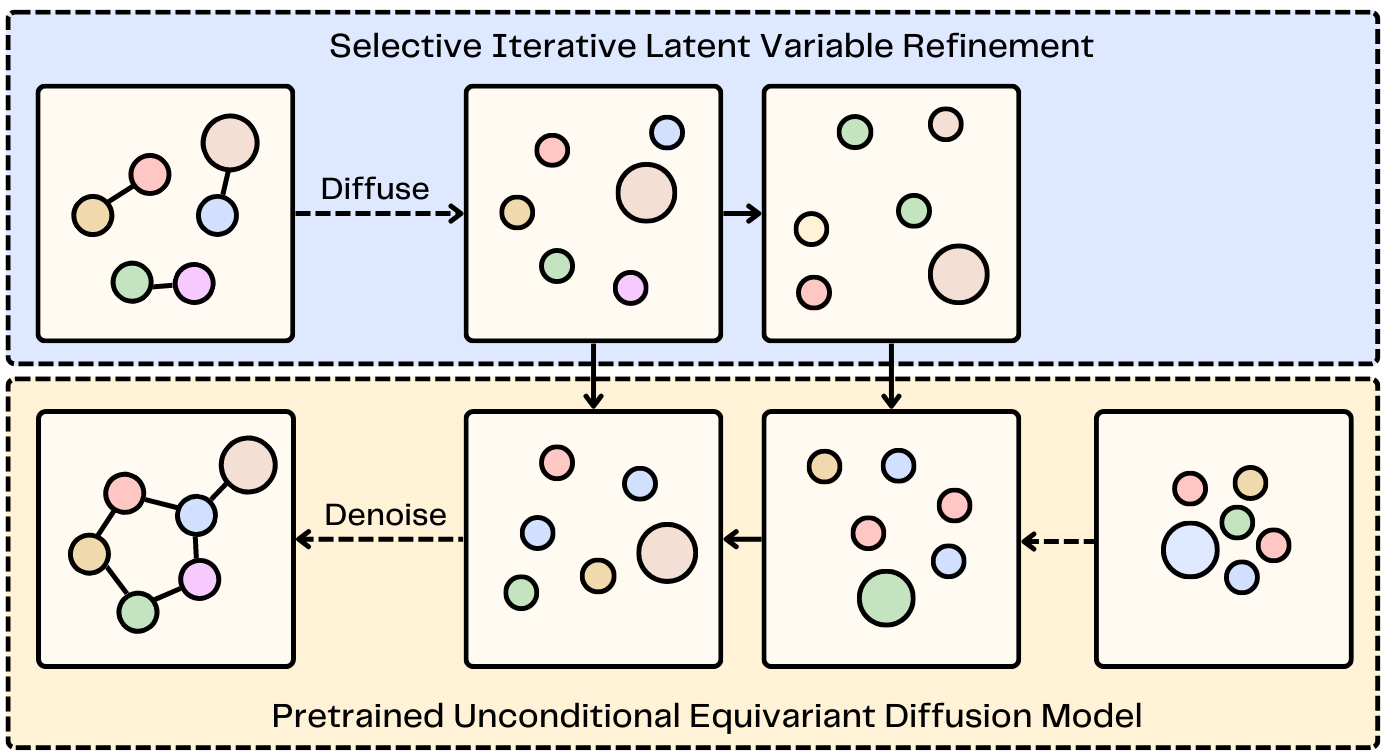
\includegraphics[width=\textwidth]{Figures/model_no_stickman.png}
    \caption{This should show the basic idea of a diffusion model}
    \label{fig:diffusion_schematic}
\end{figure}
The \textit{forward} part of the diffusion model is a Markov process, where you start out with a set of data $\mathbf{x}$ and add noise to this data over a time interval t = [0,\ldots,T] according to the following distribution:
\begin{equation}
  q(\mathbf{x_{1:T}})|\mathbf{x_0} = q(x_0)\prod_{t=1}^T q(\mathbf{x}_t|\mathbf{x}_{t-1})
\end{equation}.
The product of conditional probabilities $q(..)$ can be modelled as a Gaussian Kernel given by:
\begin{equation}
    q(x_t, x_s)=\mathcal{N}(x_t|\alpha_t/\alpha_s, \sigma_t^2-\frac{\alpha_t}{\alpha_s}\sigma^2_s
\end{equation},
for any $t>s$. The parameters $\alpha_t \in \mathbb{R}^{+}$ contains the amount of retained signal and $\sigma_t \in \mathbb{R}^+$ represents the variance and thus the amount of white noise added. 
Different people have looked at different noise schedules~\cite{sohl-dickstein2015deep, ho2020denoising}.
% Next talk about the denoising step
$\hat{p}$ is the parametric probability distribution we want to learn. 
\subsubsection*{Euquivariant diffusion model}
Unlike in image problems, the orientation of molecules matters under translations and rotations. For this purpose, we chose to equivariant diffusion model (EDM) by Hoogeboom et al.~\cite{} as our baseline generative model. The basic concept behind equivarience is that the model is invariant to rotations and translation in this case the E(3) group. This means that scalar (features such as atom types) and vector node properties (such as the positions) will be invariant to group transformations. This means that the order in which a rotation is applied does not matter. You can rotate the input to the model then apply the diffusion/denoising process and get a structure out, or you can apply the diffusion/denoising process first and then do the same rotation to get the same output. 
Mathematically this means that if we have a set of point $\mathbf{x} = (\mathbf{x}_1,\ldots,\mathbf{x}_N) \in \mathbb{^{N\times 3}}$ and each of these points has a set of scalar feature vectors $\mathbf{h}\in \mathbb{R}^{N\times k}$ associated with it these features are invariant to group transformations. The positions translations and rotations are defined according to the orthogonal matrix: $\mathbf{Rx + t} = (\mathbf{R_{x_1}+t},\ldots, \mathbf{R_{x_N}+t}$.
%%%%
% Subsection: ILVR
%%%%
\subsection{Iterative Latent Variable Refinement as a conditioning tool}
Choi et al.~\cite{choi2021ilvr} introduced a way to condition DDPMs by sampling their images from the conditional distribution $p(x_0|c)$, with the condition c:
\begin{equation}
    P_\theta(x_0|c) = \int p_\theta(x_{0:T}|c)Dx_{1:T}
\end{equation}

%%%%
% Subsection: SILVR
%%%%
\subsection{Selective Iterative Latent Variable Refinement}

\begin{algorithm}
\caption{SILVR}\label{alg:cap}
\begin{algorithmic}
\State Sample $x_T \sim \mathcal{N}(0,I)$
\For {$t$ = $T,...,1$}
    \State $z \sim \mathcal{N}(0,I)$
    \State $x_{t-1}^\prime \sim p_\theta(x_{t-1}^\prime|x_t)$
    \State $y_{t-1} \sim q(y_{t-1}^\prime|y)$
    \State $x_{t-1} \gets x_{t-1}^\prime - k x_{t-1}^\prime +k y_{t-1}$ \Comment{SILVR equation}

\EndFor
\State Sample $x,h \sim p(x,h|z_0)$ 
\end{algorithmic}
\end{algorithm}















\section{Methods}
The selective iterative latent variable refinement (SILVR) method makes use of the pre-trained equivariant diffusion model (EDM) as introduced by Hoogeboom \textit{et al.}~\cite{hoogeboom2022equivariant}. The core of the new method is the addition of a refinement process within the denoising part during run time. The resulting SILVR model produces conditional samples without any conditional training when generating new molecules. To illustrate the usefulness of this run-time modification, we show how SILVR can be used in the context of fragment-based drug design. The goal is to produce molecules that resemble a binding site based on exiting fragments and their set of atomic coordinates. 

\subsection{Conditioning the pre-trained EDM with SILVR}
The EDM by Hoodgeboom \textit{et al.} was trained on the 30 lowest energy conformations of 430,000 molecules from the GEOM dataset with explicit protons. A simplified schematic describing the EDM architecture is shared in scheme~\ref{fig:_architecture} for more details on the model theory and training refer to Hoogeboom et al.~\cite{hoogeboom2022equivariant}. This model strictly only considers atomic coordinates; all bond information is ignored. A more recent version of the EDM also accounts for bond order and SILVR could also be incorporated into this new model.~\cite{hvignac2023midi}. During training, the atomic coordinates (and their element) are passed through a forward diffusion process with iterative addition of Gaussian noise, where the extent of noise added at each step is defined by parameter $\beta$ (N.B. scheme X shows the diffusion process as a Markov chain, however in practice the state at time $t$ is determined as a direct transformation of the initial state). The diffusion process is eventually terminated when $t=T$, by which point all structure is lost and all coordinates follow a Gaussian distribution. An equivariant graph neural network (EGNN) is then trained to predict the reverse process, predicting the previous state in the sequence given any state. At run time, the generative model is instantiated with a sample from a Gaussian distribution and the series of denoising steps are applied resulting in a generated sample consisting of atomic coordinates resembling a drug-like molecule. The XYZ coordinates can then be interpreted using cheminformatics software to determine the molecular graph. 

The EDM was then adapted by introducing SILVR within the denoising process algorithm~\ref{alg:silvr}. At run time, each atom of the reference set of coordinates is mapped to an atom in the EDM. The reference coordinates are then translated such that their center of mass is at the origin. The reference coordinates are then diffused to the same timestep as that of the denoising process. That is, the amount of structure remaining from the reference should match the amount of structure formed by the generative process. A small refinement is applied to add information from the reference coordinates to the latent variable of the denoising process~\ref{eq:denoising}. This equation has the effect of shrinking the coordinates towards the origin, and then expanding the coordinates out in the direction of the reference. Importantly, the extent of this refinement is defined by the SILVR rate $r_{\mathrm{\{S}}$, with $r_{\mathrm{\{S}}=0$ providing no additional refinement and $r_{\mathrm{\{S}}=1$ will result in a total replacement of atoms. The diffusion of the reference to $t=\tau$ requires the sampling of a Gaussian; while in principle this sampling could be performed only once prior to the denoising loop, in practice better results were obtained when the Gaussian was repeatedly sampled during the denoising process. Once denoising is complete, sampled molecules can be translated back to the same coordinates as the reference by reverting the initial centre of gravity transformation; in the case of fragment data, this has the effect of returning samples to the binding site of the protein.

By introducing iterative refinement steps, the unconditional EDM can be guided to sample from a smaller region of chemical space that resembles the reference set of coordinates. Figure~\ref{fig:} demonstrates this architecture with the example of three disconnected fragments. Here, the model generates a single 5-membered ring molecule with each atom maintaining the same element, however, notice each atom has drifted slightly from the reference. This is due to the competing effects of SILVR and EDM: the EDM tries to push atoms into a chemically reasonable position, while SILVR pulls atoms towards the reference. The resulting samples, therefore, therefore resemble both valid-looking molecules and the reference set of coordinates. The ability for reference atoms of fragments to move during generation distinguishes SILVR from standard linker design~\cite{linkerdesign1, hegeboom_linker}.

\subsection{Reference Dataset: Covid-moonshot}
Reference molecules were selected from the original 23 non-covalent hits of the SARS-CoV-2 main protease (Mpro) identified by the XChem fragment screen as part of the Covid Moonshot Project~\cite{moonshot}. A more detailed picture of all fragements is presented in Figure~\ref{si:figure}. Fragments were visualised using XXX v XXX and combinations were arbitrarily selected as test cases. Fragments \textit{x0072} and \textit{x0354} were selected for benchmarking the effect of $r_{\mathrm{S}}$ on sampling; \textit{x1093}, \textit{x0072}, \textit{x2193} were selected to represent three significantly overlapping fragments; \textit{x0434}, \textit{x0305} and \textit{x0072}, \textit{x0354} were selected as partially overlapping fragments; and \textit{x0874}, \textit{x0397} were selected as two disconnected fragments, resembling a linker design type problem. Bonding information of selected fragments was deleted and XYZ coordinates were combined into a single XYZ file. Values of $r_{\mathrm{S}}$ were selected and added to the XYZ file to create a reference file containing all experiment setup information. Each experiment was sampled 1000 times. 

\subsection{Diferent observables were monitor to gauge the success of computational experiment for the generation of new models}

Different observables were used to monitor how realistic and reliable new molecules were generated and how well they can fit into the existing binding site of the SARS-CoV-2 main protease. 

\subsubsection{Atom stability}
The accuracy of placement of atoms was determined using the stability metric proposed by Hoogeboom \textit{et al.}. This metric infers bonds and bond orders between atoms by considering their interatomic distances. Once all bonds are defined, the valance of each atom is compared to its expected valance and if these values match, the atom is determined as stable. It should be noted that this metric requires the presence of all hydrogens (both explicit and implicit) for an atom to be decided as stable. For comparability with other similar published models, this metric was used unmodified. The additional metric of “molecular stability” is often reported together with atom stability (if every atom is stable then the whole molecule is stable), however as has been previously identified, large molecules sampled from this GEOM trained EDM tend to be unstable.

\subsubsection{SILVR to reference}
The SILVR algorithm creates a one-to-one mapping between reference atom coordinates and sample atom coordinates. The RMSD for this pairwise mapping, ignoring atom identities, was calculated to determine the spacial similarity of samples to the reference. 

\subsubsection{Shape similarity of sample to protein}
The agreement in the shape of samples and the main protease binding site was determined using OpenEye Tools Gaussian scoring function \textit{Shapegauss}. This scoring function measures the shape similarity between the ligand and receptor by considering each heavy atom as a Gaussian function~\cite{mcgann2003gaussian}. The most favourable score occurs “when two atoms touch but do not overlap”.  This metric does not consider any intermolecular interactions. The protein receptor file was prepared from the Mpro-x0072 crystal structure with removal of the ligand. The XYZ coordinates of samples were directly read into OpenEye Tools and the pose was re-scored with \textit{shapegauss}. 

\subsection{Maybe: Docking of molecules}


\section{Results}

\begin{figure}
    \centering
    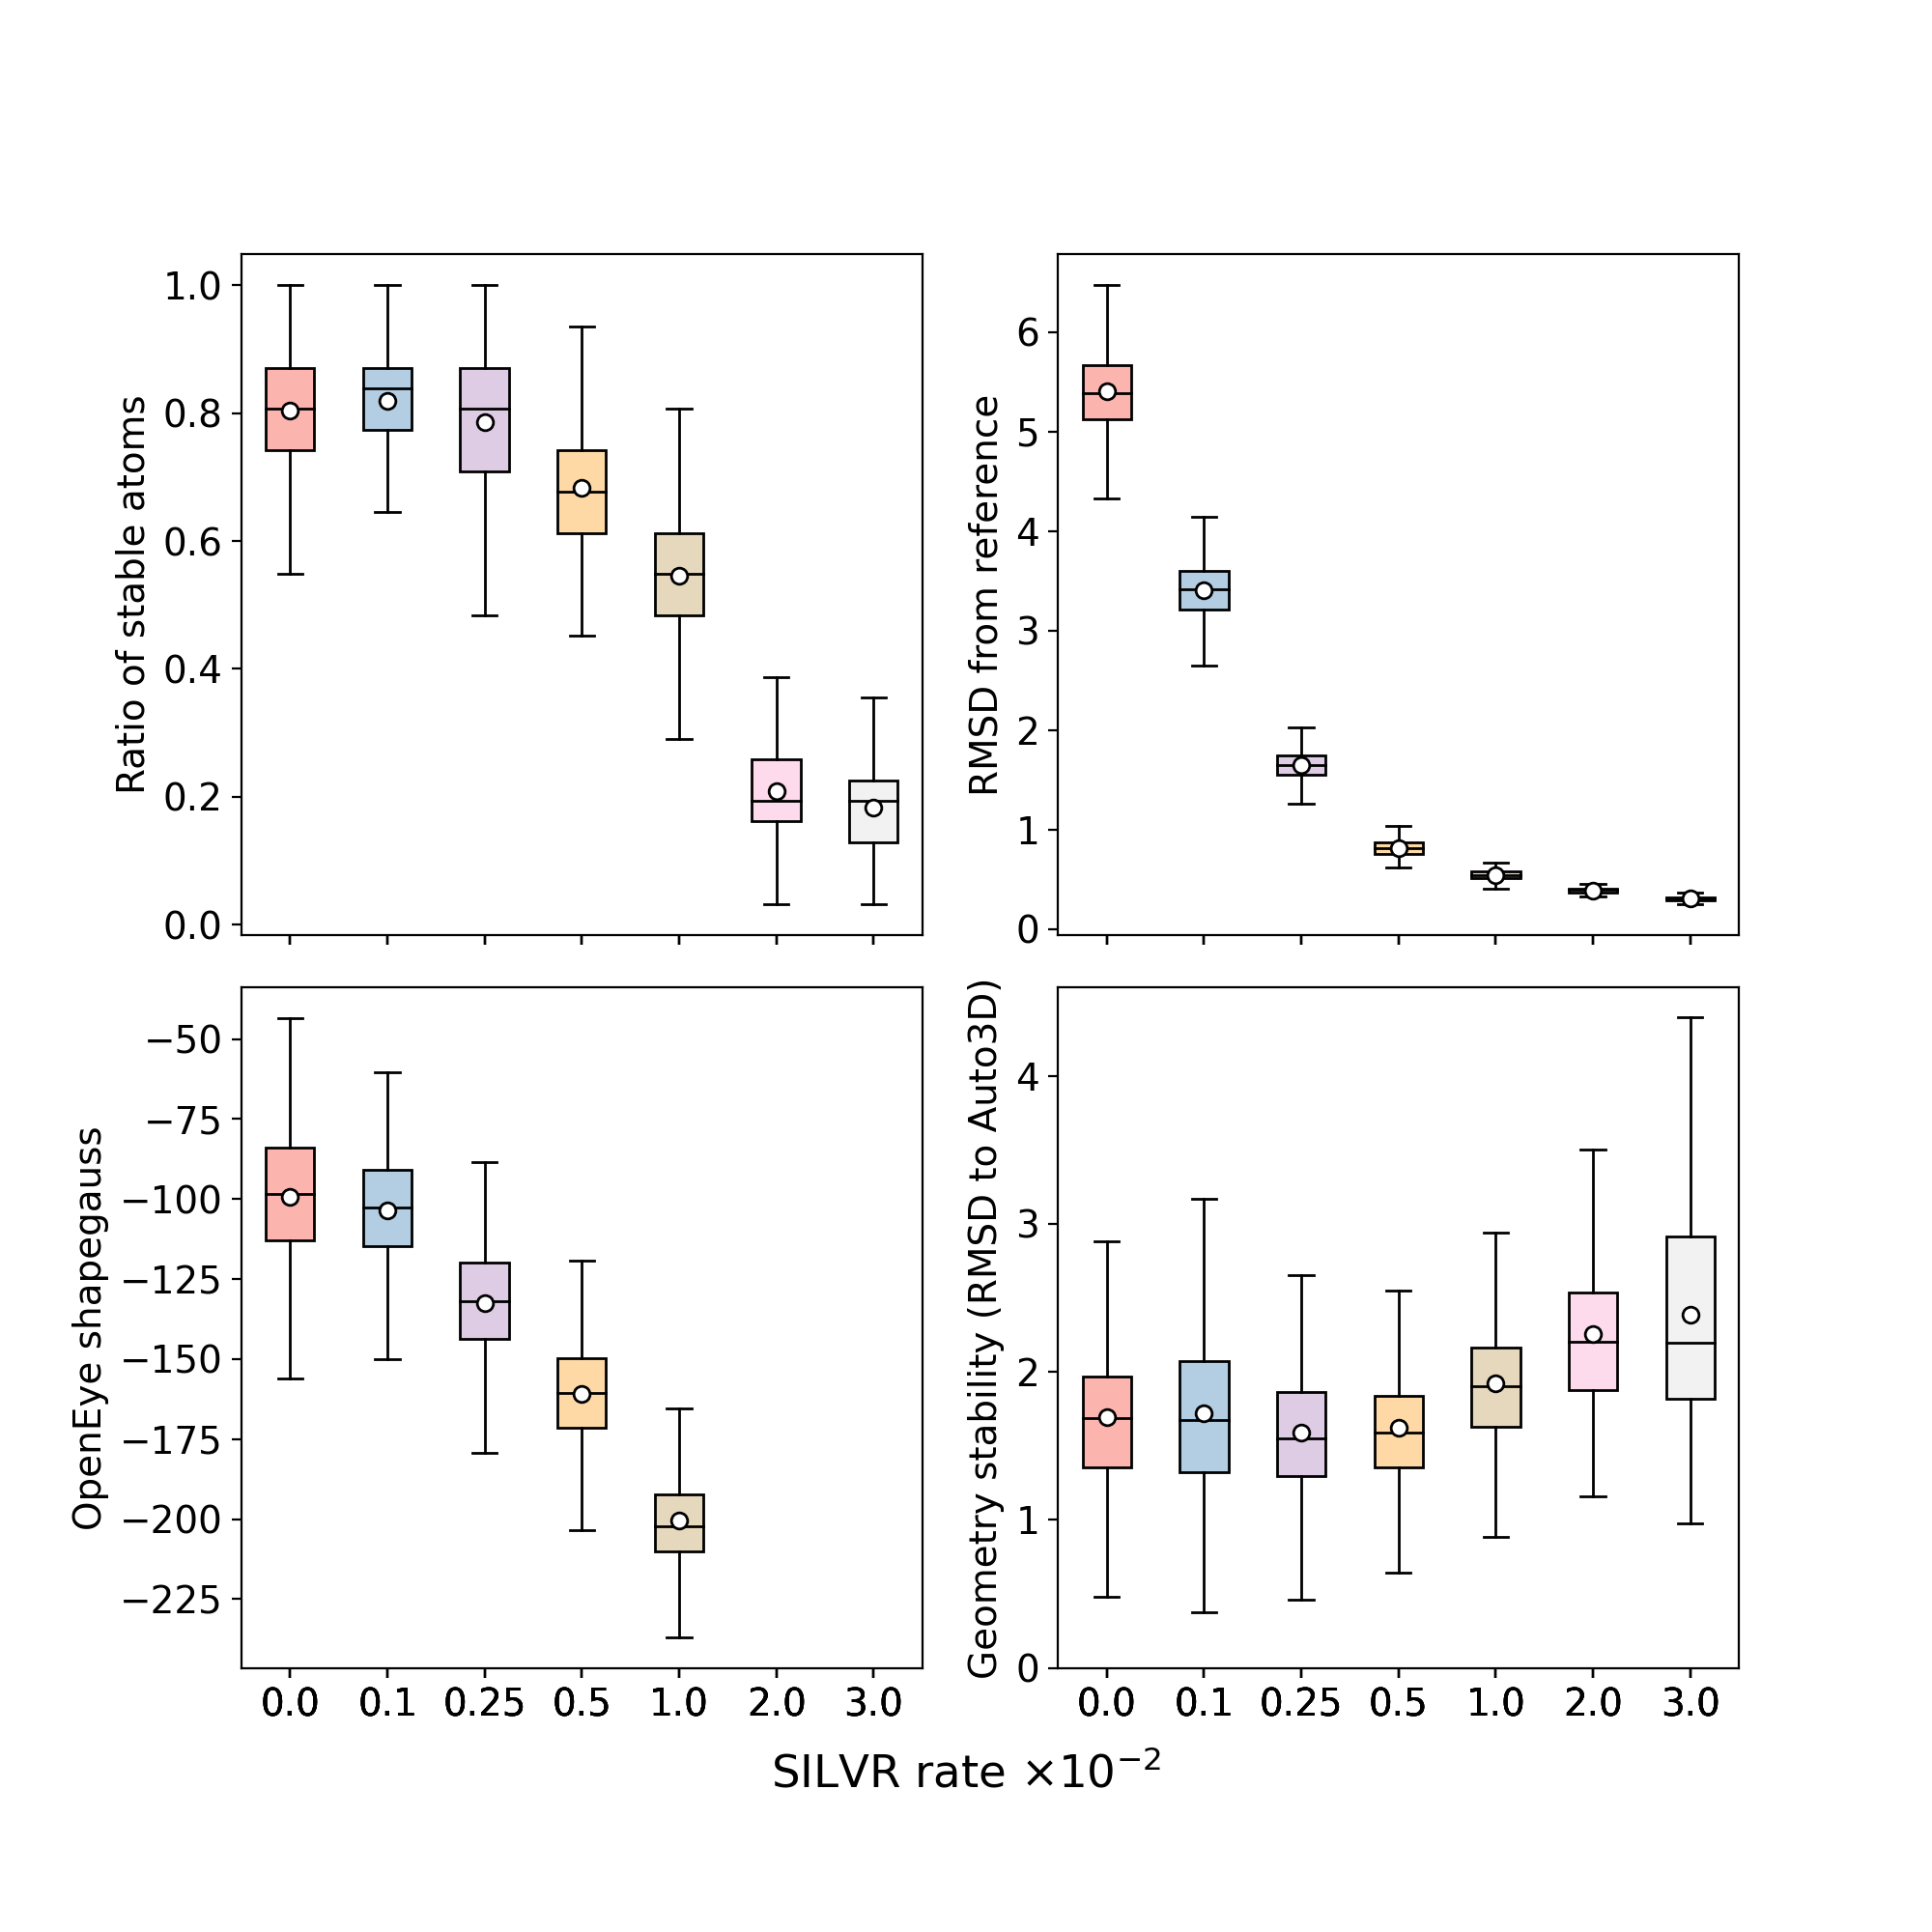
\includegraphics[width=\textwidth]{paper/Figures/Fig3/fig_3_metrics.png}
    \caption{Preliminary SILVR results (labels missing). A) Ratio of stable atoms by considering bond distances (note this includes protons but strictly maybe they should be removed. I would have to make new code for that I think). B) RMSD between samples and reference coordinated - pairwise mapping (samples rotated and translated to minimise RMSD). C)Openeye Shapegauss - still concerned I have run this wrong - lower value indicates better shape agreement with receptor D) Geometry stability - samples converted to smiles, geometry predicted using Auto3D, then RMSD with sample}
    \label{fig:metrics}
\end{figure}



\begin{figure}
    \centering
    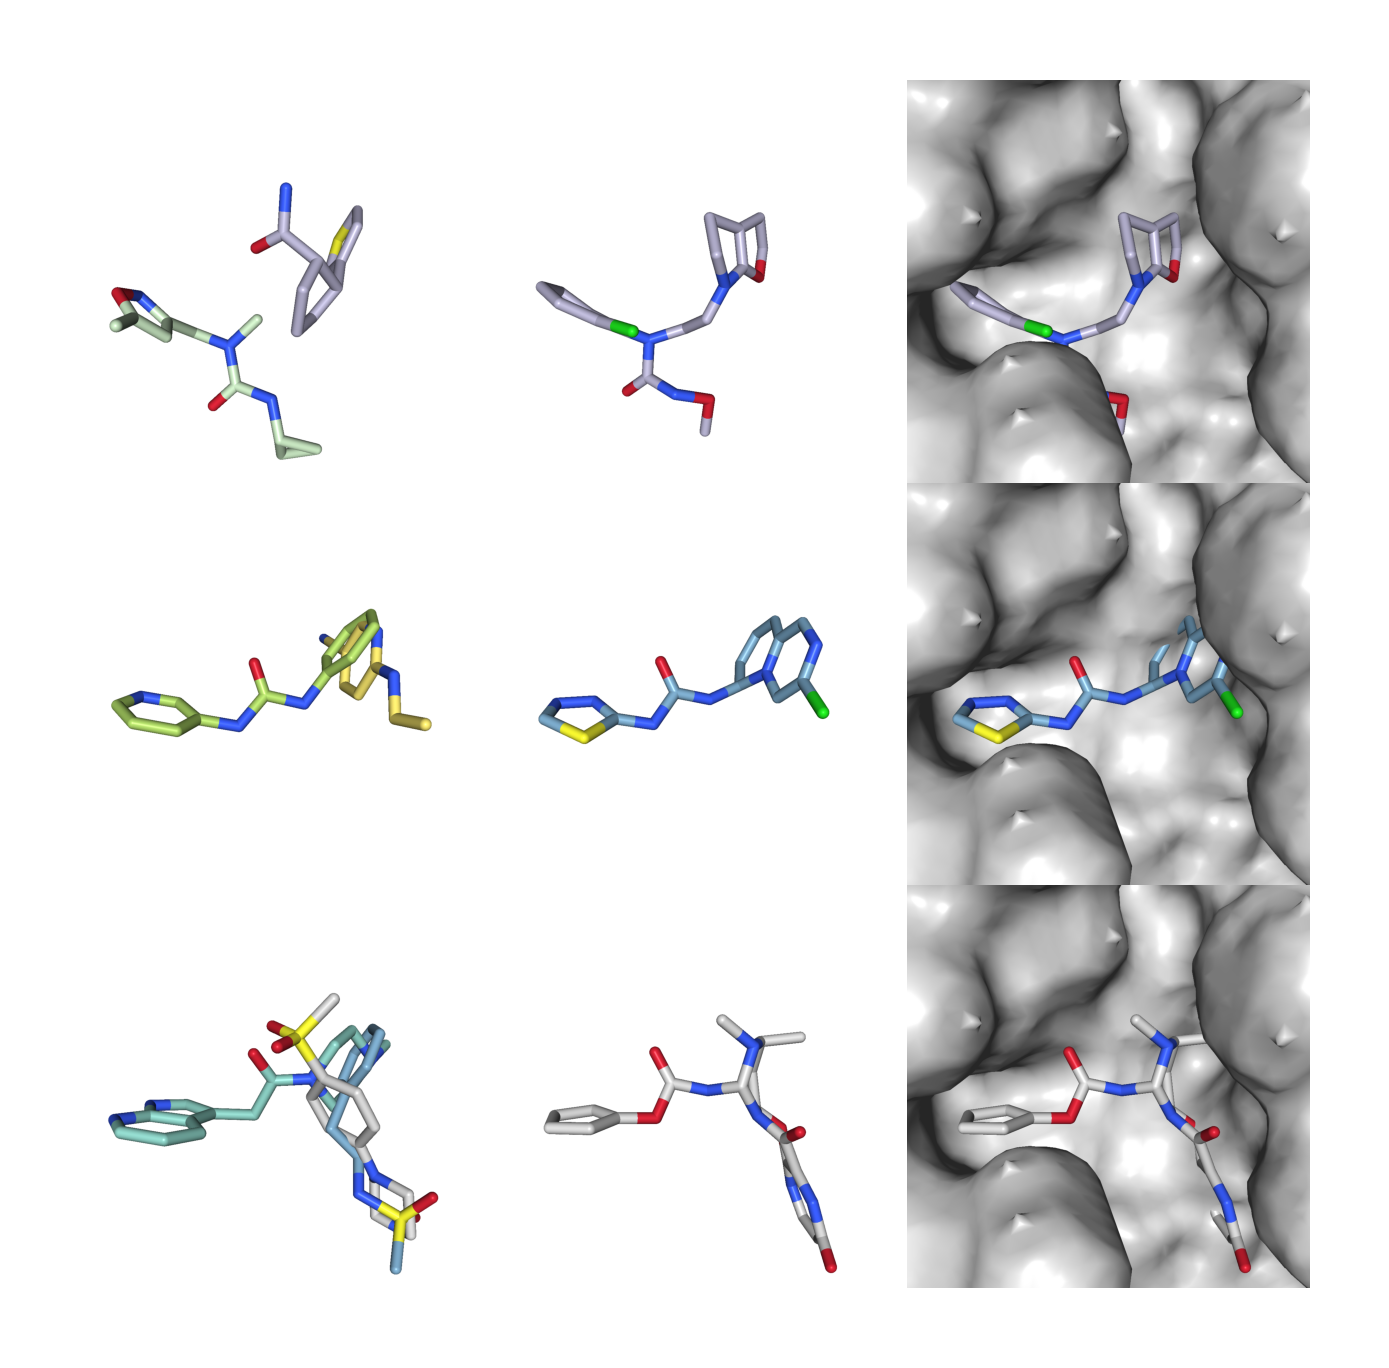
\includegraphics[width=\textwidth]{Figures/fragment_sample_bound.png}
    \caption{Examples of other reference sets and samples fitting binding site}
    \label{fig:samples}
\end{figure}


\section{Discussion and Conclusions}



%%%%%%%%%%%%%%%%%%%%%%%%%%%%%%%%%%%%%%%%%%%%%%%%%%%%%%%%%%%%%%%%%%%%%
%% The "Acknowledgement" section can be given in all manuscript
%% classes.  This should be given within the "acknowledgement"
%% environment, which will make the correct section or running title.
%%%%%%%%%%%%%%%%%%%%%%%%%%%%%%%%%%%%%%%%%%%%%%%%%%%%%%%%%%%%%%%%%%%%%
\begin{acknowledgement}
The authors thank \ldots. 

\end{acknowledgement}



%%%%%%%%%%%%%%%%%%%%%%%%%%%%%%%%%%%%%%%%%%%%%%%%%%%%%%%%%%%%%%%%%%%%%
%% The appropriate \bibliography command should be placed here.
%% Notice that the class file automatically sets \bibliographystyle
%% and also names the section correctly.
%%%%%%%%%%%%%%%%%%%%%%%%%%%%%%%%%%%%%%%%%%%%%%%%%%%%%%%%%%%%%%%%%%%%%
\bibliography{achemso-demo}

\end{document}